\documentclass[t]{beamer}
\usetheme{Berkeley}
\usecolortheme{wolverine}

\usepackage[utf8]{inputenc}
\usepackage[english,russian]{babel}

%%% Работа с картинками
\usepackage{graphicx}  % Для вставки рисунков
% \graphicspath{{images/}{images2/}}  % папки с картинками
\setlength\fboxsep{3pt} % Отступ рамки \fbox{} от рисунка
\setlength\fboxrule{1pt} % Толщина линий рамки \fbox{}
\usepackage{wrapfig} % Обтекание рисунков текстом

\author{Куценко Дмитрий} 
\title{Праздничный ужин} 
\date{\today} 

\setbeamercolor{title}{bg=}
\definecolor{links}{HTML}{BB0000}
\hypersetup{colorlinks,linkcolor=,urlcolor=links}

\begin{document}

\begin{frame}[plain]
    \titlepage
\end{frame}

\begin{frame}
    Гости будут голодные, сразу подадим поджаренные на гриле свиные ребрышки с корочкой, присыпанные луком \\
    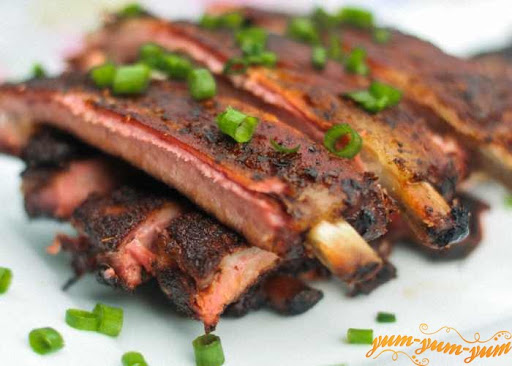
\includegraphics[width=8cm]{6-rebra.jpg}
\end{frame}

\begin{frame}
    После утоления первичного голода, подадим аутентичную пасту, ее можно есть неспешно и разговаривать \\
    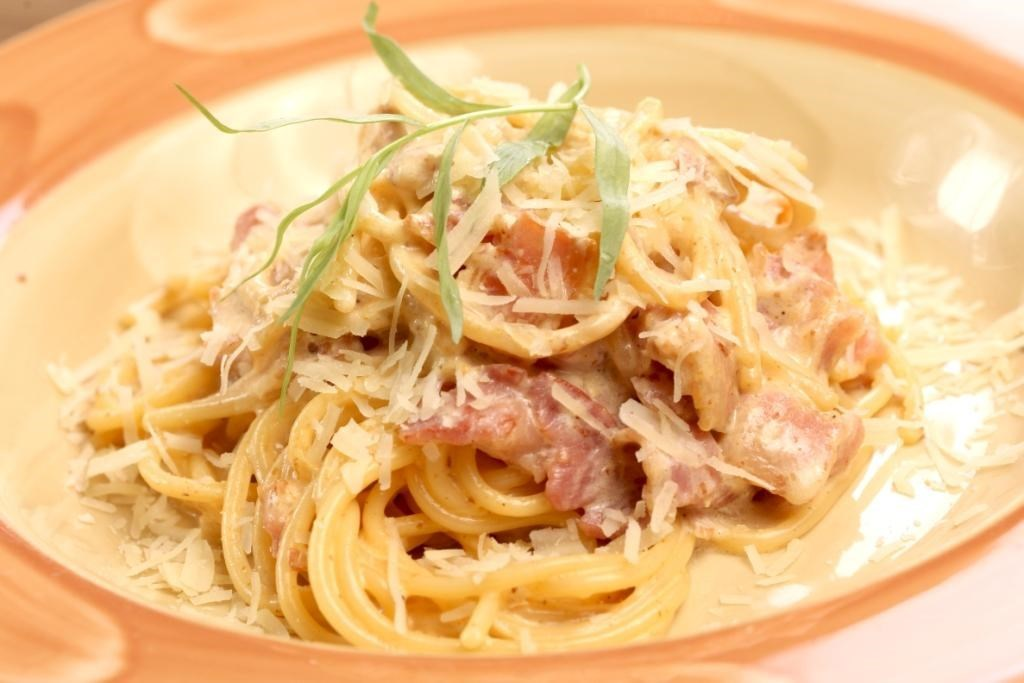
\includegraphics[width=8cm]{6-pasta.jpg}
\end{frame}

\begin{frame}
    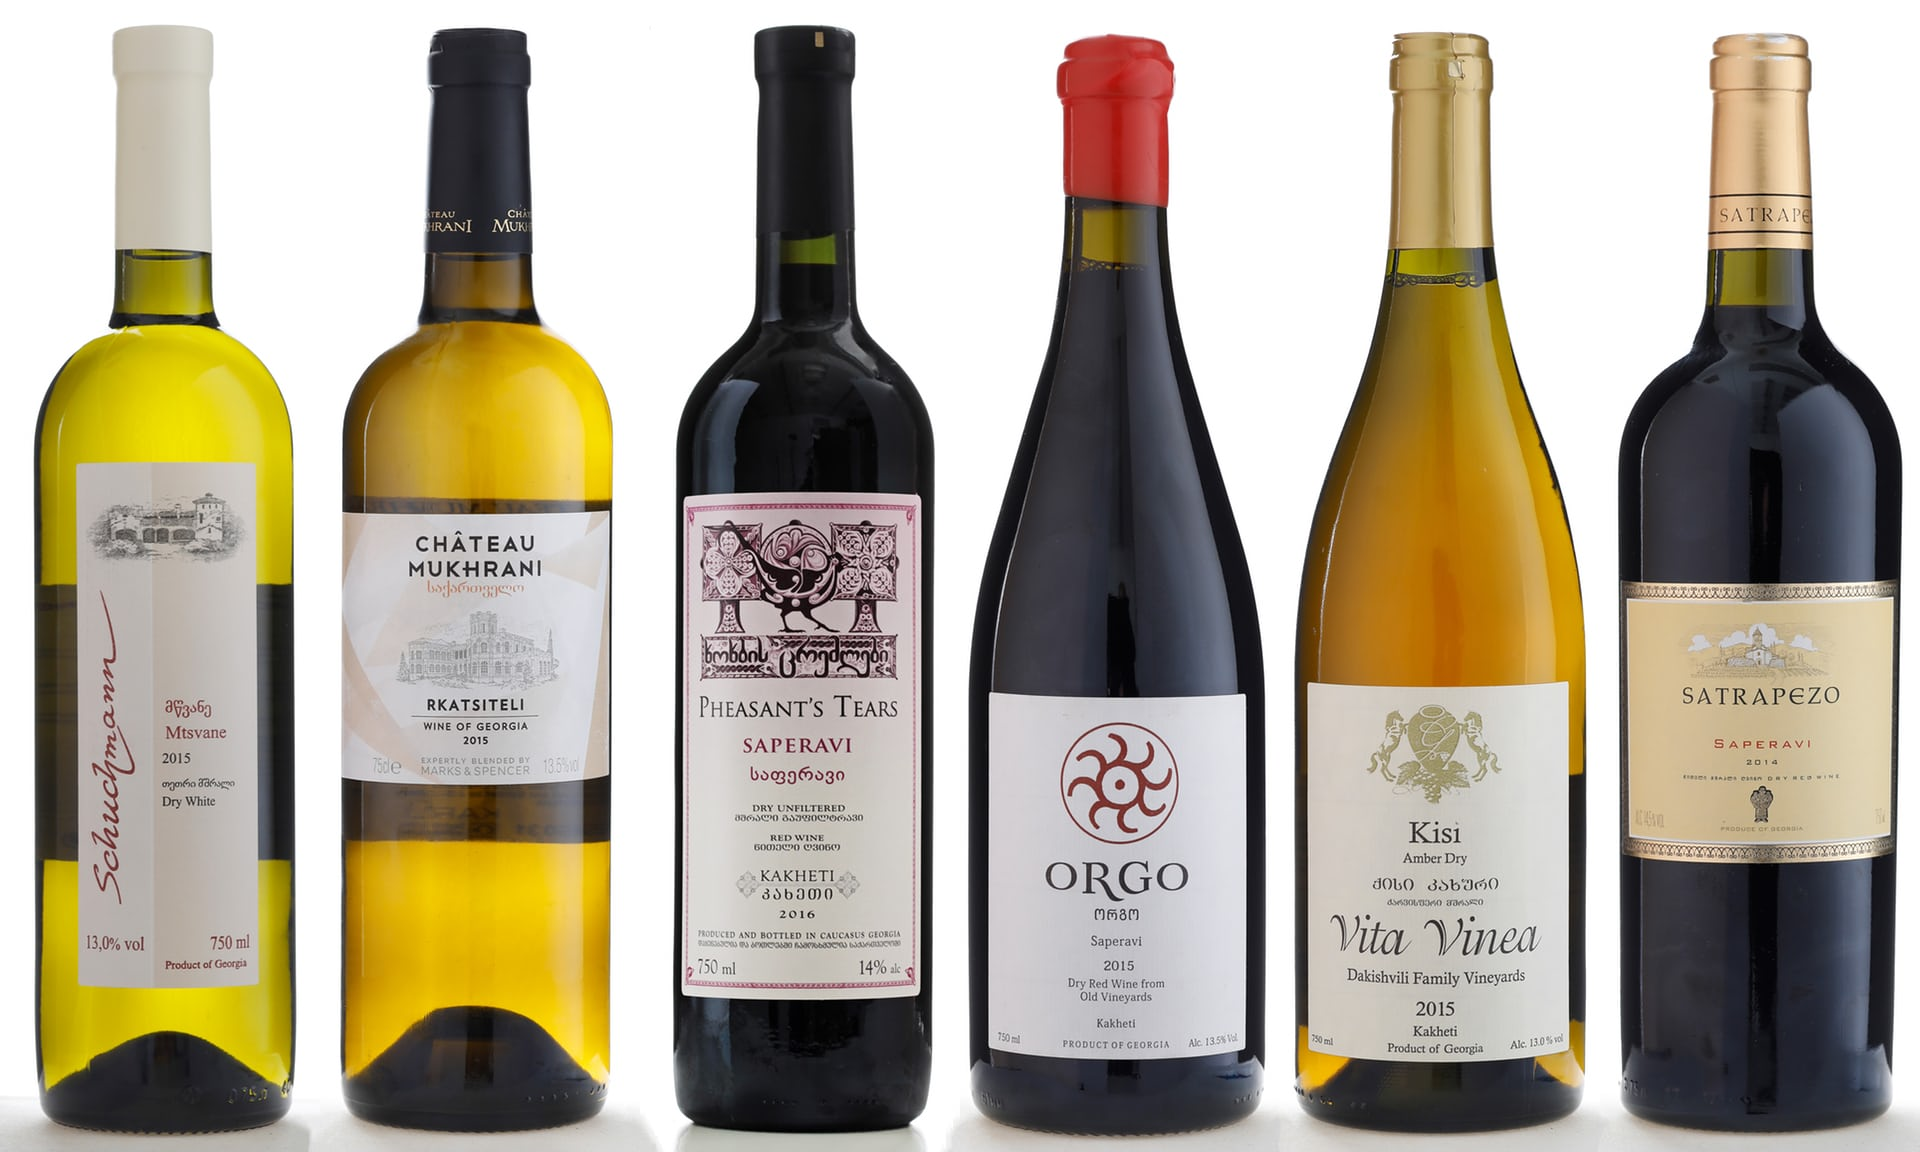
\includegraphics[width=4cm]{6-wines.jpg}
    Сразу ставим на стол вина, лучшие грузинские, можно налить и неспешно припивать:
    \begin{itemize}
        \item<1-> Белое сухое, 2015 года, от компании «Schuchmann»
        \item<2-> «Ркацители» 2015 года от «Шато Мухрани».
        \item<3-> Белое сухое, сделано в квеври компанией «Тбилвино»
        \item<4-> «Саперави» 2015 года винодельни «Слезы Фазана»
        \item<5-> «Виноградники семьи Дакишвили» - «Орго Саперави»
        \item<6-> «Вита Винеа Киси Амбер» — второе от «Дакишвили»
        \item<7-> Выдержанный в квеври «Сатрапезо Саперави» (2014)
    \end{itemize}
\end{frame}

\begin{frame}
    Пока гости едят, заказываем кальян - см. \href{https://getsmoke.ru/}{\underline{Кальяны SMOKE}} \\
    \begin{block}{Внимание!}
        Кальяны на стол ставим, только когда все перейдут на вино. С едой это совершенно не сочетается.
    \end{block}
\end{frame}

\end{document}
